\section{Magnetostatische Analyse}


\subsection{Ampèresches Gesetz}
Das Ampèresches Gesetz definiert die mathematische Verbindung zwischen


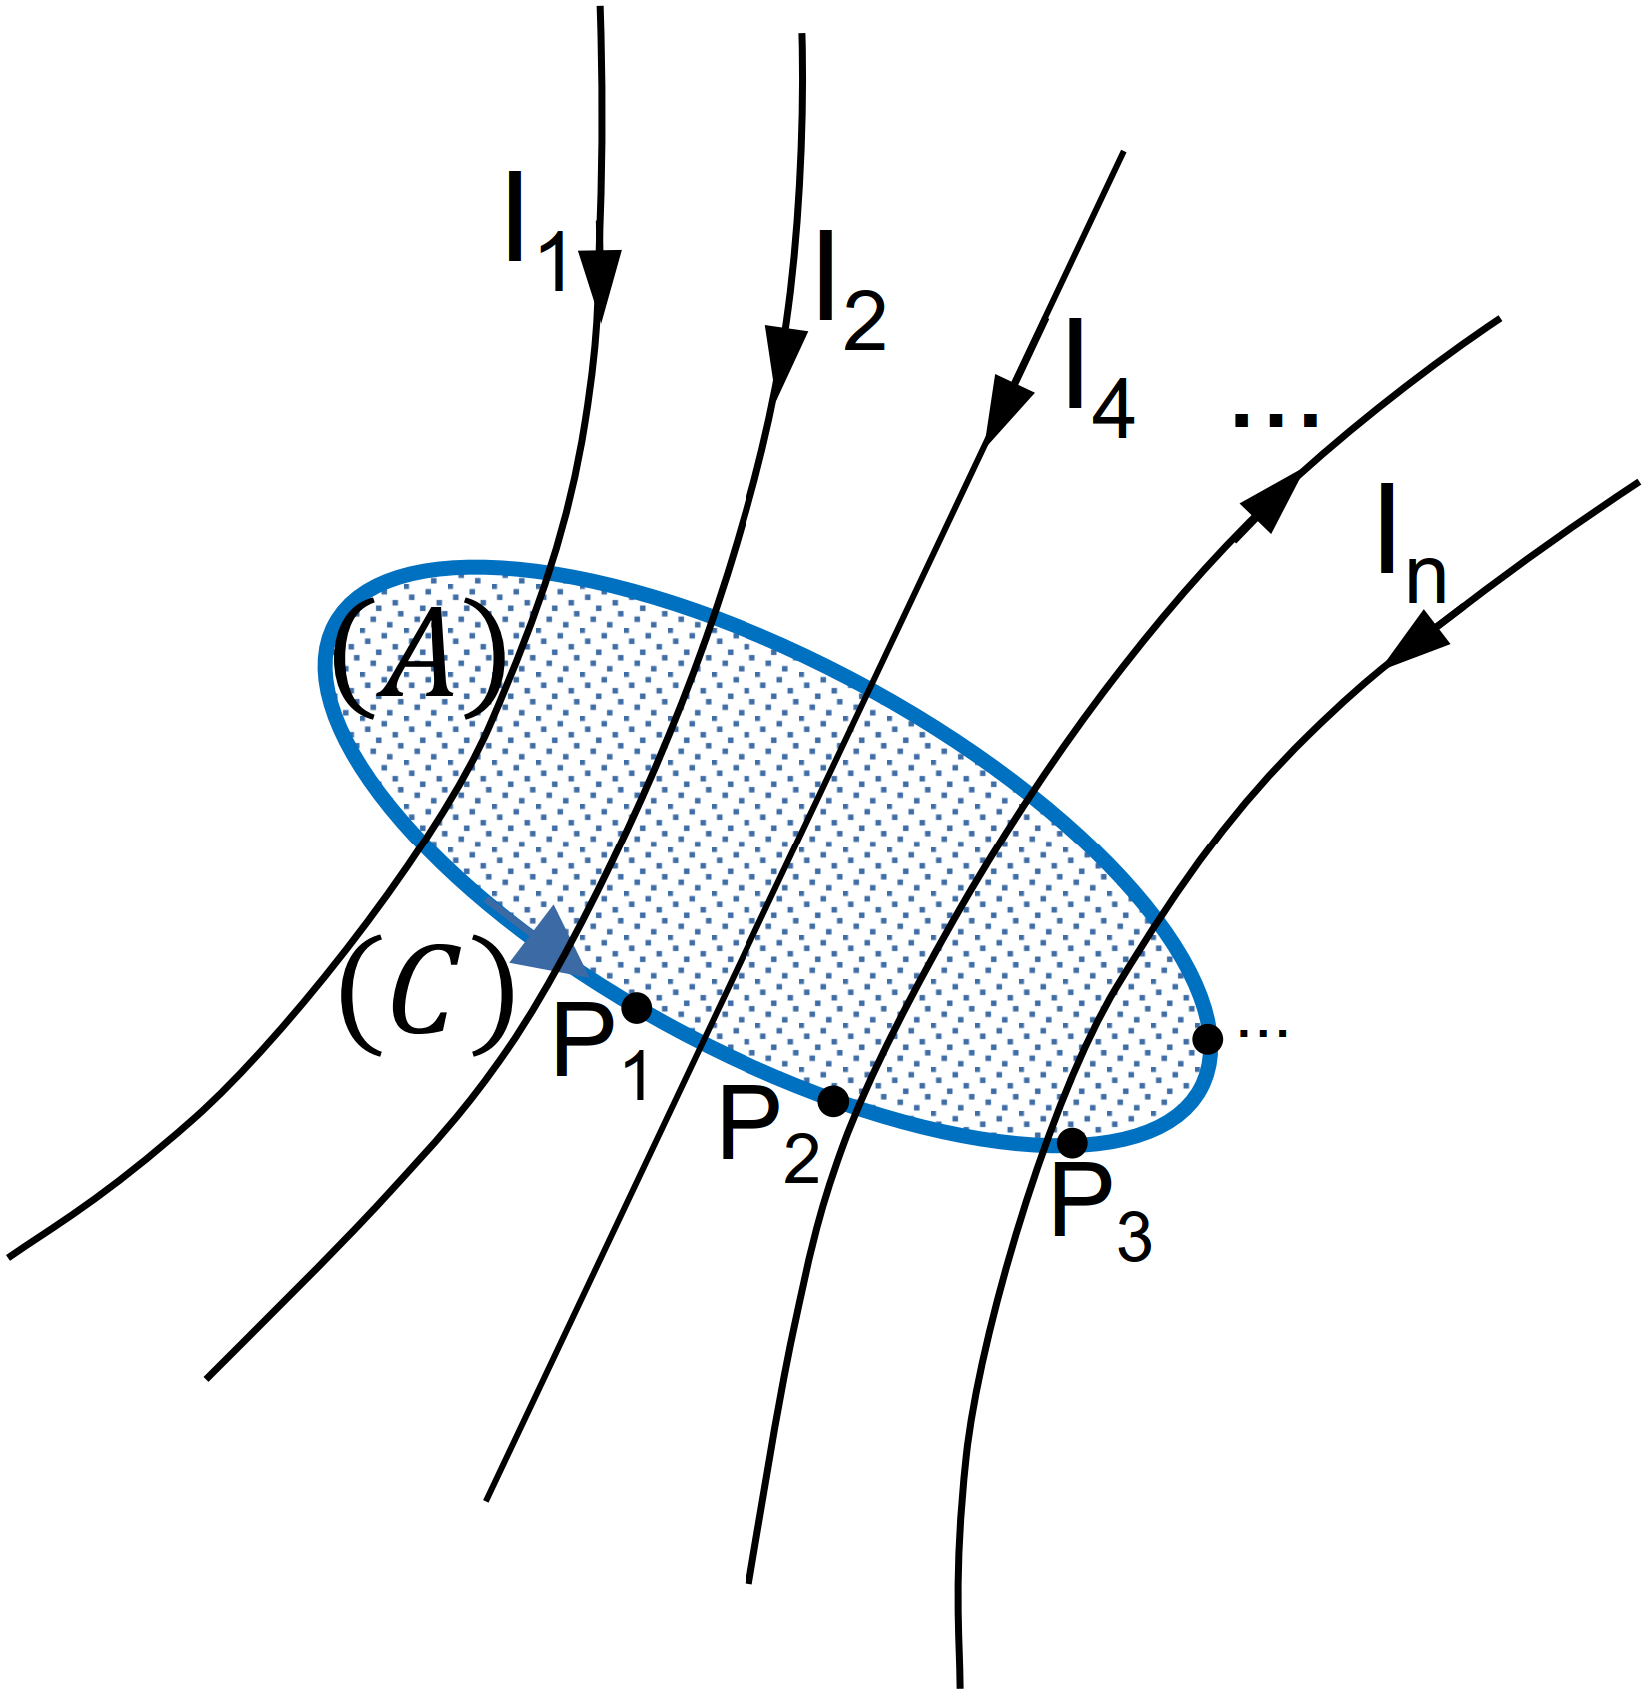
\includegraphics[width=0.5\columnwidth]{images/V3B1.png}

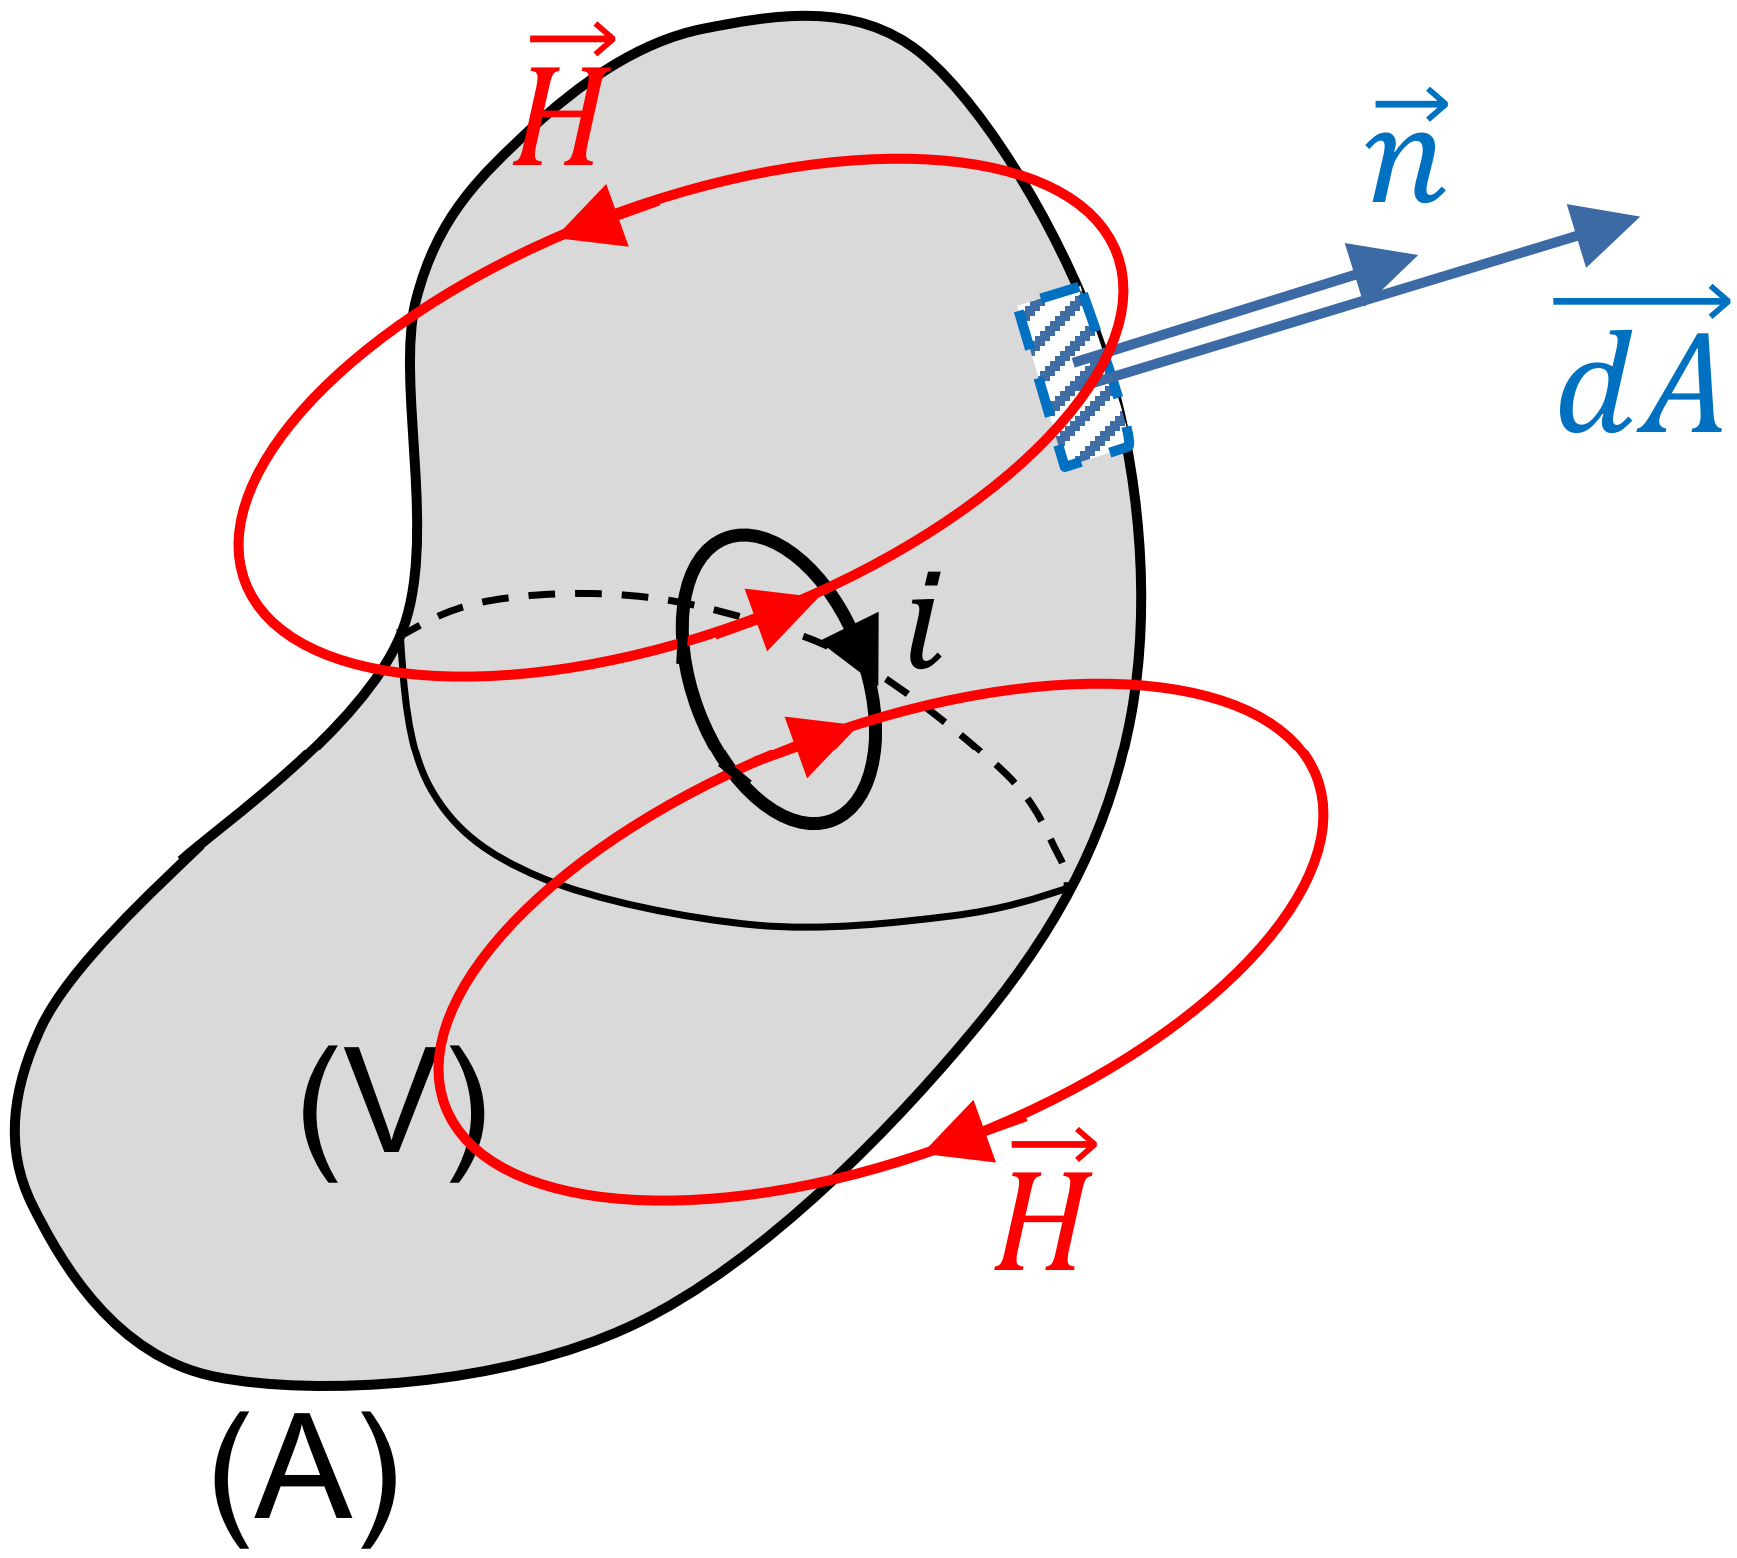
\includegraphics[width=0.5\columnwidth]{images/V3B2.png}

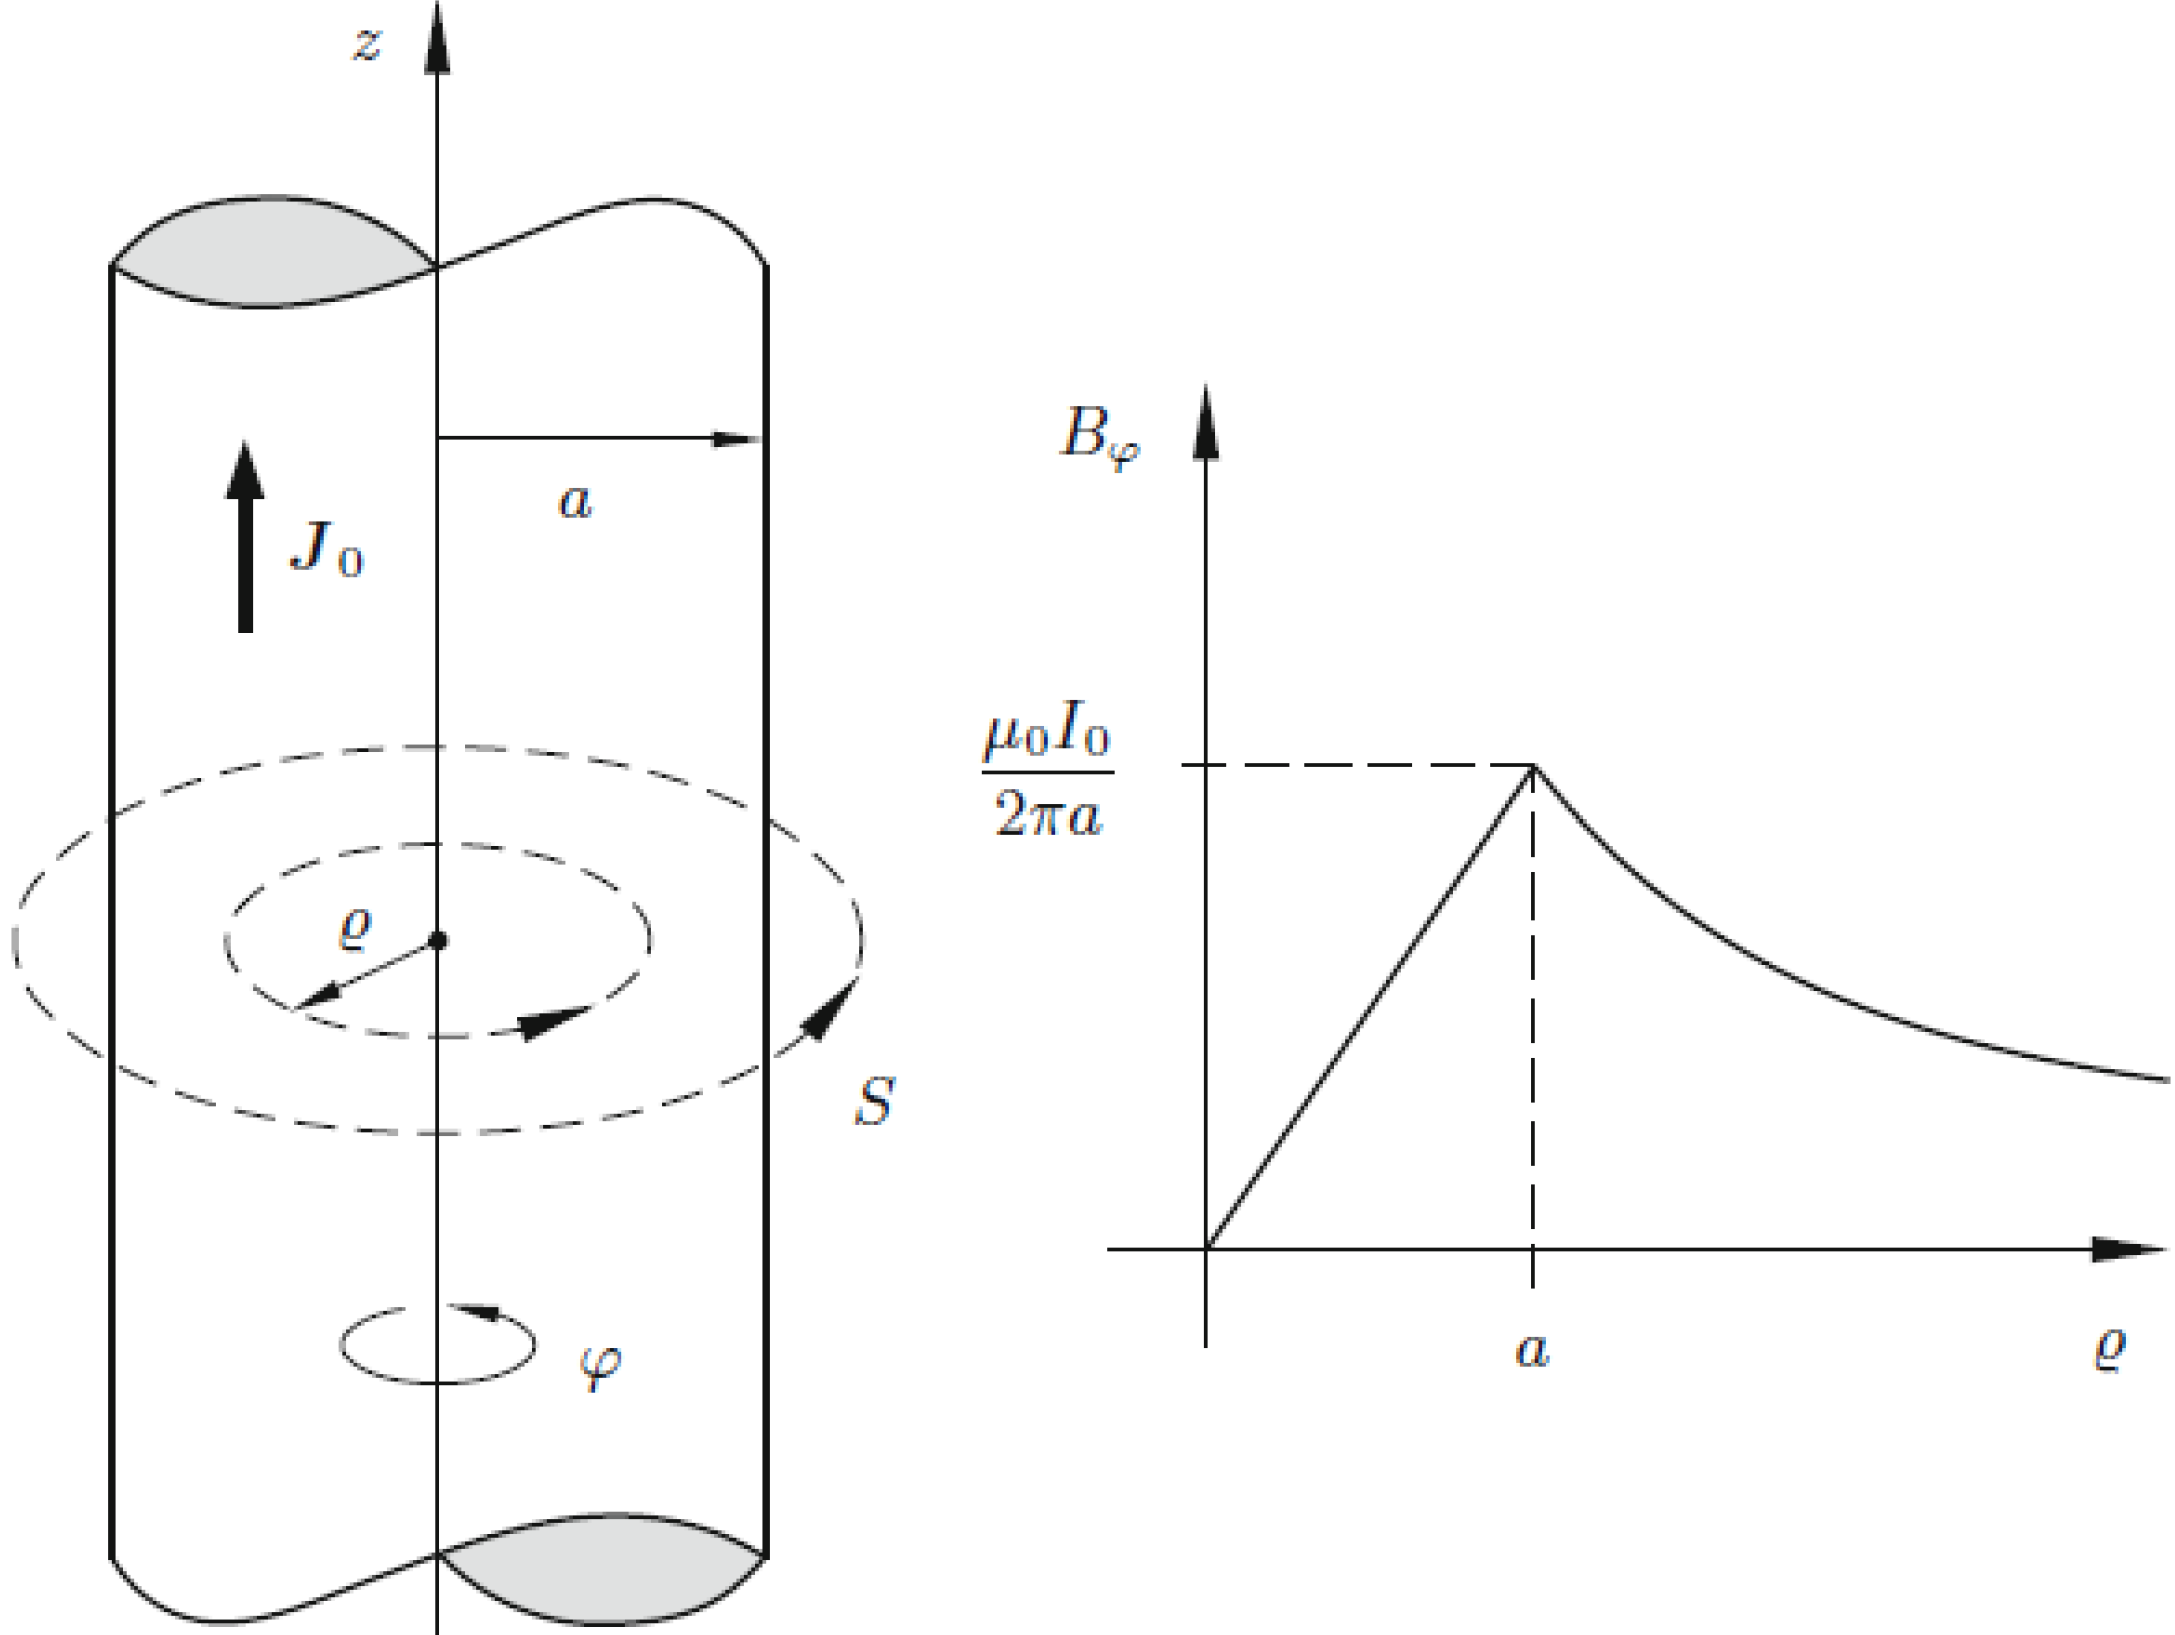
\includegraphics[width=0.5\columnwidth]{images/V3B3.png}

$\oint\limits_{(C)}\vec{H}\cdot\overrightarrow{dl}=\sum\limits_{k=1}^nI_k$

$\Theta=\sum_{k=1}^nI_k$

$\sum_{k=1}^nI_k=\iint\limits_{(A)}\vec{J}\cdot\overrightarrow{dA}$

$\oint\limits_{(C)}\vec{H}\cdot\overrightarrow{dl}=\iint\limits_{(A)}\vec{J}\cdot\overrightarrow{dA}$

$\oint\limits_{(C)}\vec{H}\cdot\overrightarrow{dl}=\iint\limits_{(A)}\vec{J}\cdot\overrightarrow{dA}$

$\oint\limits_{(C)}\vec{B}\cdot\overrightarrow{dl}=\mu_0\iint\limits_{(A)}\vec{J}\cdot\overrightarrow{dA}$

$\underset{(A)}{\operatorname*{\oiint}}\overrightarrow{B}\cdot\overrightarrow{dA}=0$

$\oint\limits_{(C)}\vec{H}\cdot\overrightarrow{dl}=\iint\limits_{(A)}\vec{J}\cdot\overrightarrow{dA}$

$\begin{aligned}
&\oint\limits_{(C)}\vec{H}\cdot\overrightarrow{dl}=\oint\limits_{(C)}(H_x\cdot dx+H_y\cdot dy+H_z\cdot dz) \\
&=\iint\limits_{(A)}\left\{\left(\frac{\partial H_y}{\partial x}-\frac{\partial H_x}{\partial y}\right)\cdot dxdy+\left(\frac{\partial H_z}{\partial y}-\frac{\partial H_y}{\partial z}\right)\cdot dydz+\left(\frac{\partial H_x}{\partial z}-\frac{\partial H_z}{\partial x}\right)\cdot dxdz\right\}
\end{aligned}$

$\oint\limits_{(C)}\vec{H}\cdot\overrightarrow{dl}=\iint\limits_{(A)}\left\{\left(\frac{\partial H_y}{\partial x}-\frac{\partial H_x}{\partial y}\right)\cdot dxdy+\left(\frac{\partial H_z}{\partial y}-\frac{\partial H_y}{\partial z}\right)\cdot dydz+\left(\frac{\partial H_x}{\partial z}-\frac{\partial H_z}{\partial x}\right)\cdot dxdz\right\}$

$\nabla\times\vec{H}=rot \vec{H}=\begin{vmatrix}\overrightarrow{e_x}&\overrightarrow{e_y}&\overrightarrow{e_z}\\\frac{\partial}{\partial x}&\frac{\partial}{\partial y}&\frac{\partial}{\partial z}\\H_x&H_y&H_z\end{vmatrix}=\left(\frac{\partial H_z}{\partial y}-\frac{\partial H_y}{\partial z}\right)\cdot\overrightarrow{e_x}+\left(\frac{\partial H_x}{\partial z}-\frac{\partial H_z}{\partial x}\right)\cdot\overrightarrow{e_y}+\left(\frac{\partial H_y}{\partial x}-\frac{\partial H_x}{\partial y}\right)\cdot\overrightarrow{e_z}$

$\oint\limits_{(C)}\overrightarrow{H}\cdot\overrightarrow{dl}=\iint\limits_{(A)}\nabla\times\overrightarrow{H}\cdot\overrightarrow{dA}$

$\oint\limits_{\begin{array}{c}(C)\\\end{array}}\vec{H}\cdot\overrightarrow{dl}=\iint\limits_{\begin{array}{c}(A)\\\end{array}}\nabla\times\vec{H}\cdot\overrightarrow{dA},\oint\limits_{\begin{array}{c}(C)\\\end{array}}\vec{H}\cdot\overrightarrow{dl}=\iint\limits_{\begin{array}{c}(A)\\\end{array}}\vec{J}\cdot\overrightarrow{dA}$

$\iint\limits_{\begin{array}{c}(A)\\\end{array}}\nabla\times\vec{H}\cdot\overrightarrow{dA}=\iint\limits_{\begin{array}{c}(A)\\\end{array}}\vec{J}\cdot\overrightarrow{dA}\Rightarrow\boxed{\nabla\times\vec{H}=\vec{J}}$

$\nabla\times\vec{H}=\vec{J}$

$\nabla\times\vec{A}=\vec{B}$

$\nabla\cdot\vec{A}=0$

$\Delta\vec{A}=-\mu_0\vec{J}$

$\vec{n}\times\vec{A}=0,(x,y,z)\in\Gamma_i$

$\vec{n}\times\overrightarrow{A_1}=\vec{n}\times\overrightarrow{A_2},(x,y,z)\in\Gamma_s$

